The hardware used to interface with neuron cultures for the cyborg is an
\textit{MEA2100} system purchased from multichannel systems. 
The MEA2100 system is built to conduct in-vitro experiments electrically active
cell cultures such as neurons.
The principal components of the MEA2100 systems are:
\subsubsection{Micro Electrode Array}
Introduced in the previous chapter, the \textit{MEA} is equipped with an array
of microscopic electrodes capable of sensing and delivering voltages to and from
nearby neurons.
\ref{fig:generic_MEA} shows an empty MEA,
\ref{st_olav_MEA} shows an MEA from st.olavs with a live neuron culture.
\subsubsection{Headstage}
The electrodes of the MEAs are measured and stimulated by the headstage which
contains the necessary high precision electronics needed for microvolt range readings.
\ref{fig:headstage} shows the same type of headstage used in this paper along
with an MEA.
\subsubsection{Interface board}
The interface board connects to up to two head-stages and is responsible for interfacing
with the data acquisition computer, as well as auxiliary equipment such as temperature
controls.
The interface board has two modes of operation.
In the first mode the interface board processes and filters data from up to two
headstages as shown in \ref{fig:IFB_regular} which can then be acquired on a normal
computer connected via USB.
In the second mode of operation a Texas instruments TMS320C6454 digital signal
processor is activated which can then be interfaced with using the secondary USB
port as shown in \ref{fig:IFB_BSP}
\begin{figure}[h!]
    %\centering
    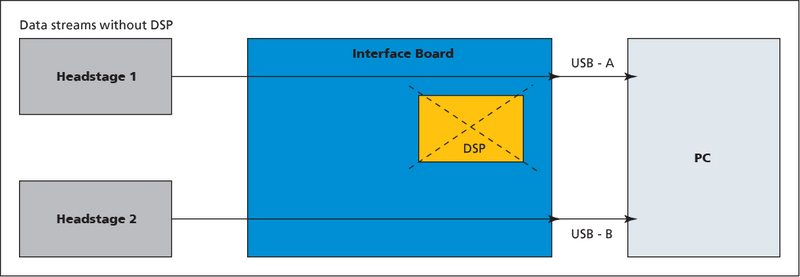
\includegraphics[width=\linewidth]{images/regular_operation.png}
    \caption{Casual mode}
    \label{fig:IFB_regular}
\end{figure}
\begin{figure}[h!]
    %\centering
    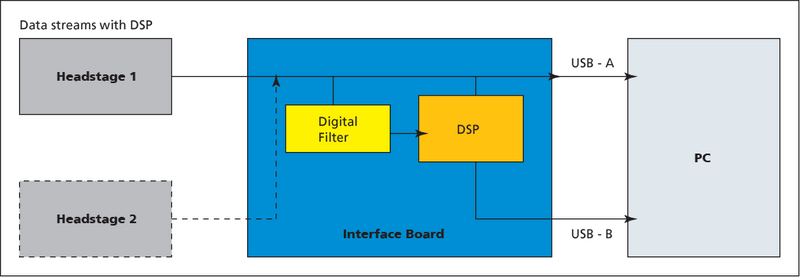
\includegraphics[width=\linewidth]{images/dsp_operation.png}
    \caption{DSP active}
    \label{fig:IFB_DSP}
\end{figure}
%%% Local Variables:
%%% mode: latex
%%% TeX-master: "../main"
%%% End: